%\clearpage
\section{PoP-level topology}


When designing or reconfiguring the physical infrastructure of an ISP, network 
operators are often guided by a design principle that emphasizes 
{\em hierarchy}~\cite{Cisco05,Gill,Morris07}.  There are two main reasons 
for implementing hierarchical network designs: {\em scalability} and {\em simplicity}.  
Compared to non-hierarchical designs, hierarchical networks can often be built at scale, 
mainly because hierarchy makes a network easier to visualize --- a key feature towards 
making it easier to manage. The situation is analogous to modularity in programming 
languages --- ideally it allows consideration of network components in isolation.

A common form of hierarchy in IP networks is based on the concept of the PoP (or 
Point of Presence). A PoP is a loosely defined term. Some providers may use the 
term to mean a physical building (housing a group of routers, switches and other 
devices), whereas others mean a metropolitan area where service is provided. 
However it is defined, though, it is a useful construct because it describes 
the logical structure of the network as the designer intended, rather than its 
particular implementation in terms of individual routers. Moreover, irrespective 
of the meaning, PoPs have an explicit geography (\eg street address or 
city/metropolitan area).  This then leads to our third major category 
of ``Internet topology'' --- the PoP-level topology.

PoP-level topologies are ideal for understanding tradeoffs between connectivity 
and redundancy, and also provide the most essential information to competitors 
or customers (about where a network is based, or who has the best access network 
in a region).  Additional reasons why the PoP-level view of networks is interesting 
include

\begin{itemize}

\item Network maps are often drawn at this level because it is an easy level 
for humans to comprehend.

\item Network optimization is often conducted at this level because the problem 
size is generally reasonable (\eg dozens of PoPs as compared to potentially 
hundreds of routers) and because inter-PoP links are much more expensive than 
intra-PoP links.

\item The internal design of PoPs is almost completely determined by simple 
templates \cite{Cisco05,Gill,Morris07}.

\item Networks change less frequently at the PoP level than at the router 
level~\cite{Shavitt10}; and

\item The PoP level is the more interesting level for many activities because 
it is less dependent on the details of protocol implementations, router vendor 
and model, and other technological details.

\end{itemize}

\begin{figure}[!thbp] 
  \begin{center}
    \begin{subfigure}[b]{0.58\textwidth}
      \centering
      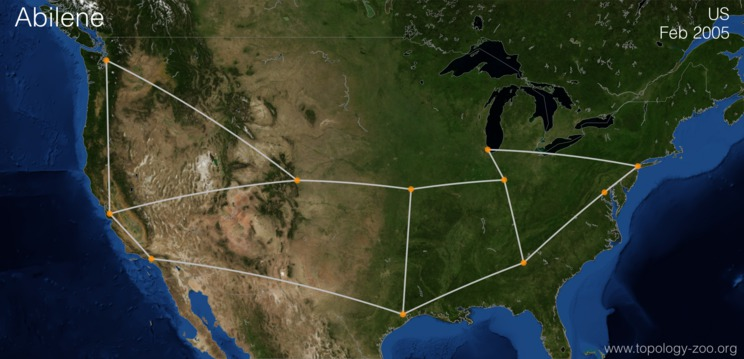
\includegraphics[width=1\textwidth]{Abilene.jpg}
    \end{subfigure}
    \hspace{0.02\textwidth}
    \begin{subfigure}[b]{0.38\textwidth}
      \centering
    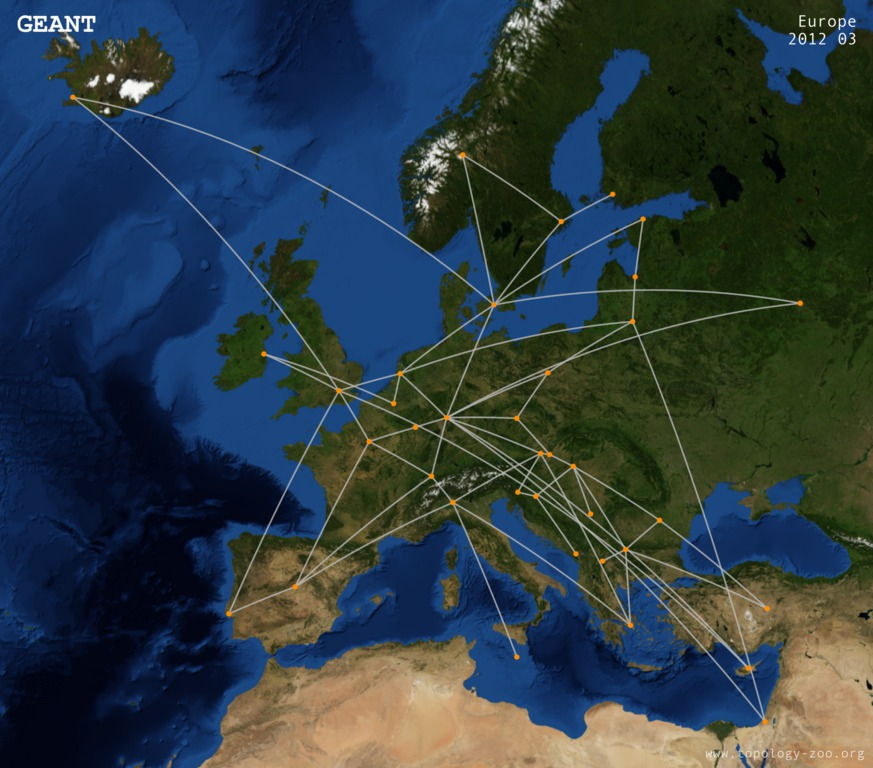
\includegraphics[width=1\columnwidth]{Geant2012.jpg}
    \end{subfigure}
    \caption{PoP-level network topologies taken from \url{www.topology-zoo.org}.
      \label{fig:pop}}
  \end{center}
\end{figure}         

The last point is subtle but important for modelling. For instance, when using a 
network as part of a simulation, one would like to have a network that is 
{\em invariant} to the method being tested. If a network designer might change 
his/her network in response to a new protocol, say a routing or traffic engineering 
algorithm, then the test will be ambiguous if it uses existing networks as models. 
PoP-level networks are less sensitive to these details than router-level networks, 
because routers impose physical and technological constraints that are almost 
completely dependent on the details of the router vendor, model and even the 
version of software running on the router.

Two examples of PoP-level topologies are depicted in \autoref{fig:pop}, 
showing the structure of two of the largest research networks (Abilene, 
and G\'{E}ANT) in the world. 

\subsection{A look back}

The study of PoP-level topologies has a briefer history than the major 
alternatives. Although the concept has existed for almost as long as networks, 
the work on modelling and measurement has typically focussed on routers (or 
their equivalent) though it is noteworthy that in simple networks (with one 
router per PoP) the two are the same. 

The first steps were taken when real data-networks were observed and
it was noted that they had structure in the form of hierarchy that was
not well represented in simple random graphs.  This observation led to
the development of \emph{structural topology
  generators}\cite{Zegura97}, based on the idea that a topology
generator should reflect the obvious hierarchical structures visible
in real networks (\eg the Georgia Tech Internetwork Topology Models
(GT-ITM)~\cite{GTITM} generator). However, this model was not
specifically aimed at modelling the PoP-level.  PoPs have been used in
more advanced structural topology generators such as
IGen~\cite{quoitin09:_igen}. IGen explicitly treats network design as
an optimization, rather than following simple stochastic rules, in
order to mimic the manner in which real networks are designed.  IGen
uses this not only for topology but also to create some of the other
important details of the network, such as the link metrics or iBGP
configurations.

The Rocketfuel project~\cite{rocketfuel_1} sought to measure (using traceroute 
with all the problems described earlier) individual ISPs, and as part of this, 
presented data and maps at the PoP level. The idea was extended by the iPlane 
project \cite{iPlane}, and by DIMES
\cite{Shavitt:2012:GIP:2238856.2238872}. However, the flaws in
traceroute make this data and the ensuing maps suspect from the start. 
However, \cite{rocketfuel_1} raised the bar with respect to validating the 
obtained PoP-level maps by trying to solicit feedback from the operators in 
charge of the mapped ISPs. 

More recently, the concept of a PoP has been explicitly used to help
guide measurement approaches, in the hope to overcome some of the
limitations of traceroute~\cite{Feldman08,Yoshida09,Shavitt10}.
However, in the absence of strong validation and given traceroute's
many problems, it is likely that most of the known issues still exist
in these approaches.

Alternatively, Knight~\etal~\cite{Zoo} have collected a set of over 
200 maps published by ISPs themselves, and transcribed these into an open 
set of data available from \url{www.topology-zoo.org}. Much of this data is 
at the PoP-level, indicating the importance of this level of network 
representation to ISPs. For a similar but complementary effort, see~\cite{atlas}.
 
\subsection{Know your measurements}

The problems in measuring PoPs are essentially the same as in any
traceroute-based survey, though it is thought (or perhaps just hoped)
that mapping IP addresses to PoPs is more straight-forward than
mapping IPs to either routers or to ASes. To the best of our
knowledge, no rigorous testing of this hypothesis has been conducted
to date, but there are some indications (\eg see \cite{Zoo}) that the
PoP-level maps provided by traceroute are no better than their router-
or AS-level counter-parts.

The topology-zoo data~\cite{Zoo}, on the other hand, is provided by
ISPs themselves and should in principle be much more accurate.
However, this dataset must also be treated carefully (as should all
data) because of potential transcription errors, or mistakes or
approximations in the maps provided by the ISPs. While such errors are
much less frequent than those encountered in measured networks, an
added concern with respect to ISP-provided maps is stale data because
there is little incentive to provide up-to-date maps.

As mentioned earlier, another important component of many PoP-level
topologies is the geographic element. Such topologies are much easier
to visualize geographically \cite{knight12:_i}, and so a frequent
interest is geolocation of the PoPs. While this is not a chapter on
geolocation, it suffices to say that many research papers have been
written on the problems of accurately mapping IP addresses to their
geolocation (\eg see \cite{Poese:2011:IGD:1971162.1971171}). Moreover,
while the routers and switches of a PoP are typically located in a
single location, city, or metropolitan area, the ``eyeballs'' (\ie end
users) connected to the PoP will be spread over some
area~\cite{rasti10:_eyebal_ases}.  However, if the researcher is
willing to diligently mine various data sources, there is hope of at
least being able to geolocate PoPs as they house potentially hundreds
or thousands of IP addresses and reside in locations with known
physical addresses (\eg carrier hotels)~\cite{atlas}.


\subsection{The nature of the PoP-level graph}

There is a common meme in network modelling that the design of a US ISP backbone 
network involves simply selecting the NFL cities, and then joining them up with 
a few lines on a map. While the real process of network design is rarely so trite, 
the picture above isn't entirely unfair. 

Most notably, PoPs are usually selected based on commercial criteria (\eg the 
desirability and size of the potential customer base in an area). So network 
engineers get little choice over the locations that they are connecting. They 
could be the NFL cities in the US, or the larger cities of another country, or 
the capitals of countries on a continent, and so on. 
Once the PoP locations have been selected, they need to be connected in some 
redundant fashion to ensure some degree of robustness to node or link failures. 
Historically, connecting these PoPs may have been done in a mostly {\em ad hoc} 
manner; see for instance \url{http://personalpages.manchester.ac.uk/staff/m.dodge/cybergeography/atlas/roberts_arpanet_large.gif}. 

However, since the burst of the Internet bubble ({\em circa} 2000), capital 
investment has become harder to obtain, and network operators and engineers 
had to justify such investment more carefully. At this point, network capacity 
started to be more carefully planned, not always using formal mathematical 
optimization, but certainly using traffic measurements to ensure less wasted 
capacity. Much of this planning and optimization is performed at the PoP-level 
simply because the router-level is much more complicated (in size, and complexity of
constraints), and because inter- and intra-PoP link costs vary by a large margin.

We have discussed network design by constrained optimization extensively in 
\autoref{sec:router} (see also references such as \cite{Li04}), and so here 
we shall only consider the main differences for PoP-level design (apart from 
those already listed above).

Perhaps the most important difference is that the physical and engineering 
constraints on a router do not directly apply for a PoP. At least in theory, 
a PoP can use as many routers as needed to provide sufficient number of ports 
for any arbitrary node degree and sufficient throughput per port. Naturally, 
the constraints in this case will arise in the form of costs, and optimization-based 
formulations of the PoP-level network design problem will feature budget constraints 
to reflect this aspect.  As budget constraints can vary greatly among different 
companies, when we look at actual PoP-level ISP backbone networks, we see a wide 
variety of designs ranging from the meshy designs with high-degree nodes only at 
the edge predicted by the HOT model, to hub and spoke like networks~\cite{Zoo}. 
In fact, the sheer variety of network designs we observe in reality suggest that 
while some network operators seem to aim at optimizing performance (given some 
lenient cost constraints), others appear to be willing to sacrifice performance 
in order to keep costs low. Moreover, network operators in different countries 
can encounter very different link costs depending on the local geographic and 
commercial environment. 

A critical but rarely discussed property of the PoP-level topology is that it 
provides the ``glue" between the more physical router-level topology on the one 
hand and the more logical AS-level topology on the other hand. Functioning as 
an ``intermediary" between these two topologies highlights the important aspect 
of the PoP-level topology that its granularity is ``just right" for many networking 
problems of practical interest --- not too coarse as to ignore important context 
(\eg the case with various AS topologies) but also not too fine as to be 
overwhelmed with unnecessary details (\eg the case with various physical 
topologies). We next discuss this property in more detail.

\subsubsection{From PoP-level to router-level connectivity}

Given a PoP-level network, there is an additional interesting
question: ``Can we map this network down to the router level?''  The
GT-ITM model addressed this through random generation of its
subnetworks, but in practice the design process of network engineers
in this case is a text-book application of repeating
patterns~\cite{Cisco05,Gill,Morris07} and hence anything but random.

The main reason for following this design process is that network 
designers often apply ``cookie cutter'' methods to design networks as a whole
or the internals of PoPs, though that term unnecessarily
trivializes the importance of repeated patterns. Repetition makes
network operations vastly simpler: the management of two PoPs requires
the same skills.  Equipment can be bulk purchased, debugging is
easier, and adding new PoPs is simpler. Finally, networks based on
templated design lead to simple design methodologies. For instance,
the inter-PoP level network topology can be optimized relatively
simply, as details such as redundancy will be supplied by the
provision of pairs of redundant routers in each PoP, with redundant
links between them.  Design often refers to the graph topology of
router interconnections, but templated design can extend to other
details, such as physical configuration within racks, connections with
external networks, or additional servers such as Domain Name Service
or Network Management Systems. 

This type of design can be mathematically described using
graph-products, though for more details, we invite the reader to consult
\cite{parsonage11:_gener_graph_produc_networ_desig_analy}.


\subsubsection{From PoP-level to AS-level connectivity: The pancake-view of the Internet}

Until now we have only really discussed the PoP-level topology of a
single network. However, there is considerable interest in how these
networks interconnect. 


The most prominent and commonly-accepted view of the Internet is as a
``network of networks'' or ASes in the AS-graph representation
discussed in \autoref{sec:as}.  A much neglected and rarely-mentioned
representation is the ``pancake view'' where we consider each network
to be a layer and where the different layers (networks) are stacked on
top of one another to form a pancake-like
structure~\cite{liljenstam03:_devel_of_inter_backb_topol}. To show
where the different networks inter-connect, we add links across
layers; intra-network connectivity is shown as links within each
layer.  For a set of ``peer'' networks, one advantage of this pancake
view is that these networks often cover similar geographic areas and
inter-connect in multiple locations, but at a limited set of cities
(determined either by where private interconnects are seen as
commercially viable, or where IXPs are available). Importantly,
depending on the types of networks, many of them host their PoPs in
one and the same commercial colocation facilities whose street
addresses are generally known\footnote{One problem in establishing
  such a view lies in the limitations of current IP geolocation
  services \cite{Poese:2011:IGD:1971162.1971171}.}.  As such, the
pancake view allows one to visualize not only this connectivity inside
and between such providers but also the geography of their PoP-level
topologies.

However, as far as we are aware, there has been no significant work
studying this pancake view together with the different inter-connections, 
other than noting that it exists. The dearth of studies and models perhaps 
stems from the problems in obtaining the measurements necessary for constructing
this view (see the discussions in \autoref{sec:as}), but it is
perhaps one of the most interesting areas for future Internet topology research.
 

\subsection{A look ahead}

We have focused in this section and the earlier sections mostly on traditional ISPs
or network service providers which operate networks that have more or
less pronounced backbones and cover geographic areas ranging from 
individual countries to entire geographic regions to the entire globe.
However, there are many other networks that are not ISPs and consist of PoPs
without their own physical infrastructures to connect them (\eg content
providers, CDNs, Web-hosting companies). The PoPs of these networks are
typically located in commercial colocation facilities or data centers
that are operated by third-party companies for the explicit purpose of 
interconnecting such infrastructureless networks among one another or 
with ISPs or network service providers. 

The importance of the role of such dedicated Internet infrastructure
in the form of colocation facilities is best illustrated with a
concrete example.  As of December 2012, Equinix \url{www.equinix.com},
one of the leading companies in global interconnection and data
centers, owned and operated in 14 countries in 5 continents some 30
colocation facilities. In these 30+ colocation facilities that are
located in the major cities around the world, more than 4,000 networks
connected directly to their customers and partners.

Another largely under-researched topic concerns the fact that in this chapter,
we treated router-, PoP-, and AS-level topologies as static objects, when in
reality, they evolve over time.  In particular, it is rarely the case that
a network operator designs a new network from scratch.  Network design typically
has to include as important aspects awareness and knowledge of the 
existing network that the operator intends to change due to, for example,
drastic changes in the traffic demand that the original network design can
no longer handle efficiently.

In view of these an other added challenges, the PoP-level view promises
to be one of the more useful and interesting direction for future Internet
topology research.  In particular, measurements and models at this level have
considerable scope for the future, and extensions of HOT-like optimization
models may provide much more realistic synthetic networks than are
currently available. At the same time, work on interconnection of networks 
at this level also provides considerable scope, but will require significant
advances in our ability to measure and model the flow of traffic across the
different networks as it is the traffic that ultimately determines much of
the structure and evolution of the different topologies that we discussed 
in this chapter.

\subsection{Notes}

The primary source for the material presented in this section (and a
much lengthier discussion of many of the issues) is

\begin{itemize}
\item[\cite{Zoo}] S.Knight, H.Nguyen, N.Falkner, R.Bowden, M.Roughan,
  The Internet topology zoo. IEEE Journal on Selected Areas in
  Communications (JSAC) 29, 9, 1765-1775, October 2011.

\end{itemize}

\noindent For additional and more in-depth reading materials (in
addition to the references indicated throughout) we point to

\begin{itemize}

\item[\cite{Shavitt:2012:GIP:2238856.2238872}] Y.Shavitt and
  N.Zilberman, Geographical Internet PoP-level maps. In Proceedings of
  the 4th international conference on Traffic Monitoring and Analysis
  (Berlin, Heidelberg), TMA'12, Springer-Verlag, pp. 121-124, 2012.

\item[\cite{parsonage11:_gener_graph_produc_networ_desig_analy}]
  E.Parsonage, H.Nguyen, R.Bowden, K.Knight, N.Falkner, M.Roughan,
  Generalized graph products for network design and analysis. In 19th
  IEEE International Conference on Network Protocols (ICNP)
  (Vancouver, CA), October 2011.

\item[\cite{Shavitt10}] Y.Shavitt and N.Zilberman, A structural
  approach for PoP geo-location. In IEEE Infocom 2010.

\item[\cite{Yoshida09}] K.Yoshida, Y.Kikuchi, M.Yamamoto, Y.Fujii,
  K.Nagami, I.Nakagawa and H.Esaki, Inferring PoP-level ISP topology
  through end-to-end delay measurement. In PAM, pp. 35-44, 2009.

\end{itemize}

